\documentclass[12pt]{article}
\usepackage{graphicx} % For including images/logo
\usepackage{geometry} % For custom margins
\usepackage{fancyhdr} % For custom headers/footers
\usepackage{titling}  % For custom title formatting
\usepackage{amsmath}  % For advanced math formatting
\usepackage{amssymb}  % For additional math symbols
\usepackage{enumitem} % For custom enumeration
\usepackage{xcolor}   % For text coloring
\usepackage{circuitikz}

% Set margins
\geometry{a4paper, margin=1in}

% Title, name, and date
\title{\textbf{EE1200 - ELECTRIC CIRCUITS LAB}}
\author{EE24BTECH11012 - Bhavanisankar G S \\ EE24BTECH11019 - Dwarak A}
\date{\today}

% Add logo to the title
\pretitle{%
    \begin{center}
    
\includegraphics[width=0.5\textwidth]{IITH.png} \\ % Replace with your logo file
    \vspace{1cm} % Adjust spacing as needed
    \LARGE
}
\posttitle{\end{center}}

\begin{document}

% First page with title, name, date, and logo
\maketitle
\thispagestyle{empty} % Remove page number from the first page

\newpage

\section{Find the RC circuit response with all three cases below for square wave input, and plot the output and input for a transient response for the first five cycles and steady-state response as well. \\
	RC == T \\ RC $>>$ T \\ RC $<<$ T}

\subsection{\textbf{AIM :}} \\
To find the RC circuit response with square wave input and plot the output and input for transient response for the first five cycles and steady state response.

\subsection{\textbf{APPARATUS REQUIRED :}} \\
\begin{itemize}
\item A digital function generator
\item A Cathode Ray Oscilloscope
\item Connecting wires
\item A resistance ( $1 k\Omega$ )
\item A capacitor ( $1 \mu F$ )
\item Oscilloscope probe
\end{itemize}

\subsection{\textbf{THEORY : }}
\begin{itemize}
\item RC circuit consists of a resistor (R) and capacitor (C) connected in series. When a square wave input is applied to such a circuit, the response is determined by the charging and discharging behaviour of the capacitor and the associated time constant ( $\tau$ ).
\item Time constant for a series RC circuit is the product of the magnitude of Resistance and capacitance.
\begin{align}
	\tau = R C
\end{align}
\item Voltage across the capacitor varies as
\begin{align}
	V_{C} (t) &= V_{0} \left( {1 - e^{\frac{-t}{\tau}}} \right) \text{ for charging } \\
	V_{C} (t) &= V_{0} e^{\frac{-t}{\tau}} \text{ for discharging }
\end{align}
\item For \textbf{High frequency input} ( RC $<<$ T ), the capacitor has enough time to almost fully charge and discharge during each cycle. Hence, the voltage across the capacitor closely resembles the input with rounded edges due to exponential charging/discharging.
\item For \textbf{Low frequency input} ( RC $>>$ T ), the capacitor does not have enough time to fully charge or discharge. Hence, the voltage across capacitor appears as a triangular waveform with reduced amplitude.
\end{itemize}

\subsection{\textbf{PROCEDURE : }}
\begin{itemize}
\item Connect the RC-circuit as shown in \eqref{fig:fig}.
\begin{figure}[h!]
    \centering
    \begin{circuitikz}
        % Define circuit components
        \draw 
        (0,0) node[ground]{} % Ground symbol
        (0,0) to[square voltage source, l=\(5V\)] (0,3) % Square wave voltage source
        to[R, l=$1 k\Omega$] (3,3) % Resistor
        to[C, l=$1 \mu F$] (3,0) % Capacitor
        -- (0,0); % Closing the circuit
    \end{circuitikz}
    \label{fig:fig}
    \caption{RC Circuit with a 5V Square Wave Input}
\end{figure}

\item Input a square wave of amplitude 5 V from the function generator, with time period equal to $RC$. The corresponding output is captured from the CRO.
\item The experiment is repeated for two more values of frequency such that $RC >> T $ and $RC << T$, and capture them.
\item The figures are then compared with those created by python.
\end{itemize}

\subsection{\textbf{VERIFICATION : }} \\
\begin{itemize}
\item $RC << T$ :
We have 
\begin{align}
	V &= V_{0} \left( 1 - e^\frac{-t}{\tau} \right)
\end{align}
Substituting $t = 2.44 s, R = 1000 \Omega, C = 1 \mu F$, we have
\begin{align}
	V &\approx 5.0
\end{align}
\item $RC == T$ :
Substituting $t = 740  \mu s, R = 1000 \Omega, C = 1 \mu F$, we have
\begin{align}
	V &\approx 3 V
\end{align}
\item $RC >> T$ :
We have 
\begin{align}
	V &= V_{0} \left( 1 - e^\frac{-t}{\tau} \right)
\end{align}
Substituting $t = 220 \mu s, R = 1000 \Omega, C = 1 \mu F$, we have
\begin{align}
	V &\approx 2.5 V 
\end{align}
\end{itemize}

\subsection{\textbf{FIGURES : }} \\

\begin{figure*}[!htb]
    {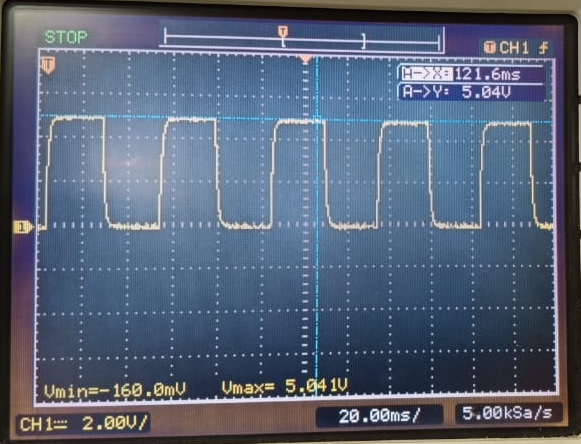
\includegraphics[ width=0.31\textwidth]{5.png}}
    \hspace{\fill}
    {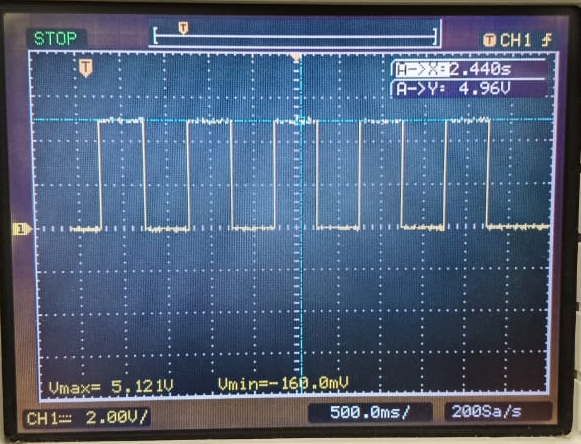
\includegraphics[ width=0.31\textwidth]{6.png}}
    \hspace{\fill}
    {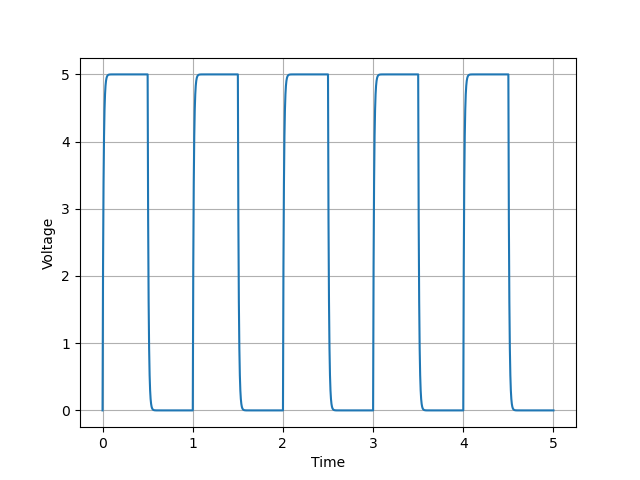
\includegraphics[ width=0.31\textwidth]{fig1.png}}\\
    \caption{$ RC << T $}
\end{figure*}

\begin{figure*}[!htb]
    {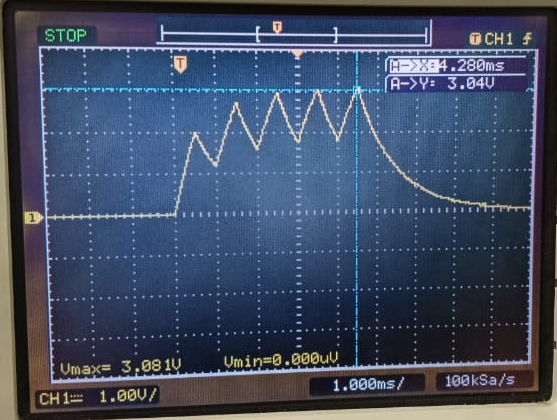
\includegraphics[ width=0.31\textwidth]{3.png}}
    \hspace{\fill}
    {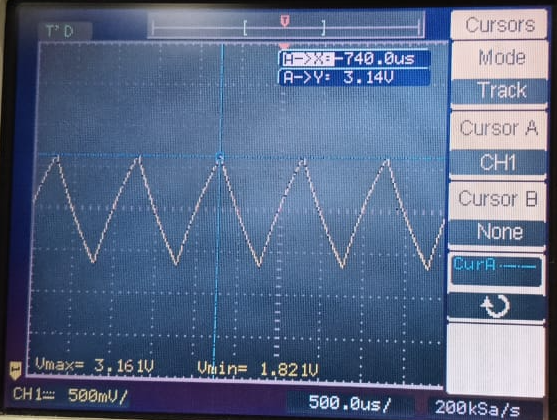
\includegraphics[ width=0.31\textwidth]{4.png}}
    \hspace{\fill}
    {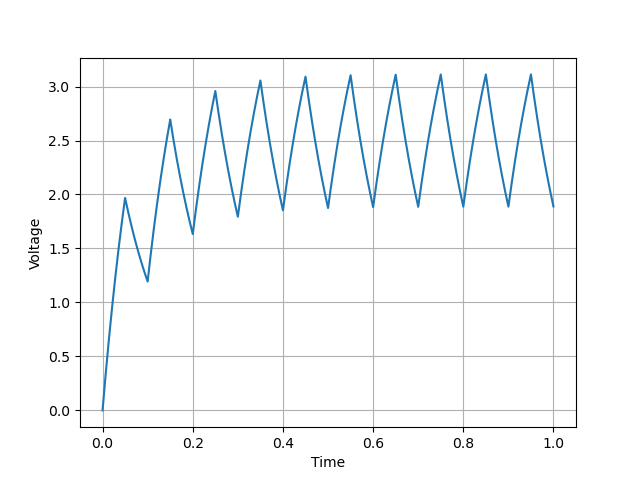
\includegraphics[ width=0.31\textwidth]{fig2.png}}\\
    \caption{$RC == T $}
\end{figure*}

\begin{figure*}[!htb]
    {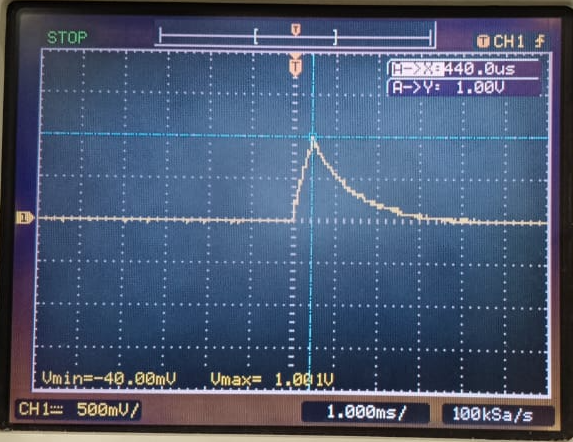
\includegraphics[ width=0.31\textwidth]{1.png}}
    \hspace{\fill}
    {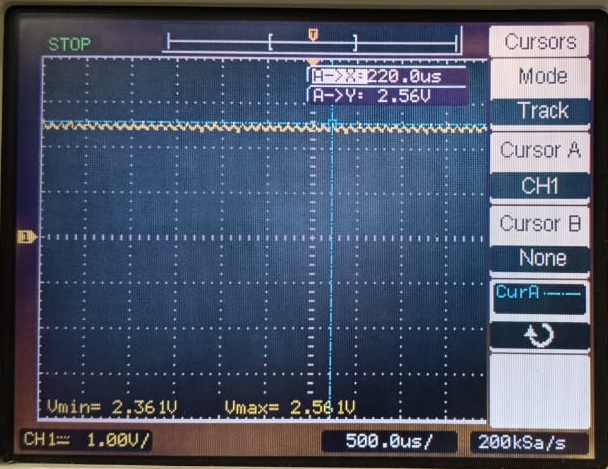
\includegraphics[ width=0.31\textwidth]{2.png}}
    \hspace{\fill}
    {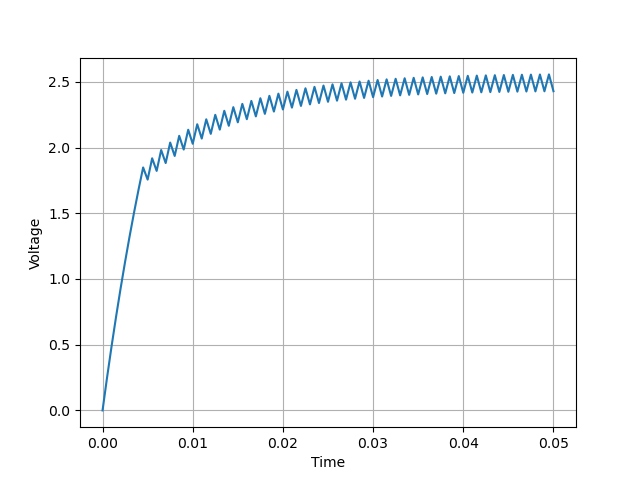
\includegraphics[ width=0.31\textwidth]{fig3.png}}\\
    \caption{$RC >> T$}
\end{figure*}


\end{document}
